%%%%%%%%%%%%%%%%%%%%%%%%%%%%%%%%%%%%%%%%%%%%%%%%%%%%%%%%%%%%%%%%%%%%%%%
% Thema: Poster
% Autor: Musterman
% Datum: 12.05
%%%%%%%%%%%%%%%%%%%%%%%%%%%%%%%%%%%%%%%%%%%%%%%%%%%%%%%%%%%%%%%%%%%%%%%
%
\documentclass[a0,27pt,portrait]{a0poster}
%\documentclass[portrait,a0,posterdraft]{a0poster}
\pagestyle{empty}
\renewcommand{\figurename}{Abb.}
\renewcommand{\tablename}{Abb.}
%
%%%%%%%%%%%%%%%%%%%%%%%%%%%%%%%%%%%%%%%%%%%%%%%%%%%%%%%%%%%%%%%%%%%%%%%
% Paket zum Erzeugen der Spalten
\usepackage{multicol}
\usepackage{siunitx}
%%%%%%%%%%%%%%%%%%%%%%%%%%%%%%%%%%%%%%%%%%%%%%%%%%%%%%%%%%%%%%%%%%%%%%%
% Eingabekodierung
\usepackage[utf8]{inputenc}
\usepackage[T1]{fontenc}
\usepackage{ae} %wenn Ulaute nicht gehen
\usepackage{graphicx}
%\usepackage{subfigure}
\usepackage[ngerman]{babel}
\usepackage[hang]{caption}
\usepackage{floatrow}
\usepackage{multirow}
\addto\captionsngerman{\renewcommand{\figurename}{Fig.}}
%\addto\captionsngerman{\renewcommand{\subfigurename}{\sf }}
\addto\captionsngerman{\renewcommand{\tablename}{Tab.}}

%\begin{übler Trick um die Orinalüberschrift zu unterdrücken}
\addto{\centeringsngerman}{\renewcommand*{\refname}{}} %Literaturüberschfit unterdrücken
%\ende{übler Trick}
\usepackage[%
style=ieee,   
defernumbers=true,      % to set different numeric types -e.g. A1...A2 B1...B2
sortcase=false,%		% false- keine unterscheidung zwischen gross und kleinschrift 
bibencoding=utf8,%
doi = false, 
isbn = false,
subentry=true,
url = false,  
backend=biber,
maxcitenames=2,
mincitenames=1,
]{biblatex}				% um 8-bit zeichen zu erkennen, fuer umlaute
%%%%%%%%%%%%%%%%%%%%%%%%%%%%%%%%%%%%%%%%%%%%%%%%%%%%%%%%%%%%%%%%%%%%%%%
% für Farbe
\usepackage{color}
\definecolor{darkgreen}{rgb}{0,0.5,0}
\definecolor{darkblue}{rgb}{0,0,0.5}

%%%%%%%%%%%%%%%%%%%%%%%%%%%%%%%%%%%%%%%%%%%%%%%%%%%%%%%%%%%%%%%%%%%%%%%
% Mathepaket
\usepackage{amsmath}

%%%%%%%%%%%%%%%%%%%%%%%%%%%%%%%%%%%%%%%%%%%%%%%%%%%%%%%%%%%%%%%%%%%%%%%
% Ist für Boxen (wie das hier benutzte Ovalbox) zuständig
\usepackage{fancybox}

%%%%%%%%%%%%%%%%%%%%%%%%%%%%%%%%%%%%%%%%%%%%%%%%%%%%%%%%%%%%%%%%%%%%%%%
% Graphikpaket, ermöglicht png, jpg und pdf bilder
\usepackage{graphicx}

%%%%%%%%%%%%%%%%%%%%%%%%%%%%%%%%%%%%%%%%%%%%%%%%%%%%%%%%%%%%%%%%%%%%%%%
% Seiteneinstellungen
\renewcommand\baselinestretch{1.35}
\parskip=0.5\baselineskip

\parindent0mm %Einrücktiefe der ersten Zeile eines Absatzes
\topmargin-1cm
\marginparwidth0mm

%Ränder rechts/links
\oddsidemargin+10mm
\evensidemargin+10mm
\textwidth770mm
%\textheight1140mm

%%%%%%%%%%%%%%%%%%%%%%%%%%%%%%%%%%%%%%%%%%%%%%%%%%%%%%%%%%%%%%%%%%%%%%%
% Eigene Definitionen zur Erleichterung des Satzes
\newcommand{\spaltenbreite}{25}   % Spaltenbreite für Bilder
\newcommand{\bildbreite}{25cm}    % Einheitliche Bildbreite

%%%%%%%%%%%%%%%%%%%%%%%%%%%%%%%%%%%%%%%%%%%%%%%%%%%%%%%%%%%%%%%%%%%%%%%
% Box- und Spalteneinstellungen
\setlength{\fboxrule}{3.25mm} 	%Definiert die Linienstärke für nachfolgende fbox- und framebox-Befehle
\setlength{\fboxsep}{5mm}		%Abstand zwischen Rahmen und Text bei den /fbox und /framebox Befehlen.
\setlength{\columnsep}{15mm}	%Spaltenabstand
\setlength{\columnseprule}{0pt}	%Balken zwischen Spalten {0pt}->keine Balken

%%%%%%%%%%%%%%%%%%%%%%%%%%%%%%%%%%%%%%%%%%%%%%%%%%%%%%%%%%%%%%%%%%%%%%%
% Einheitslänge für picture-Umgebungen
%\setlength{\unitlength}{1.0cm}
\unitlength1cm

%%%%%%%%%%%%%%%%%%%%%%%%%%%%%%%%%%%%%%%%%%%%%%%%%%%%%%%%%%%%%%%%%%%%%%%
% Grafikpfad, hier liegen alle Bilder
%\graphicspath{{images/}}

%%%%%%%%%%%%%%%%%%%%%%%%%%%%%%%%%%%%%%%%%%%%%%%%%%%%%%%%%%%%%%%%%%%%%%%
% Zaehler fuer lineale. Sie werden gebraucht, wenn das Linealmacro included wird
\newcounter{skalax}
\newcounter{skalay}

%%%%%%%%%%%%%%%%%%%%%%%%%%%%%%%%%%%%%%%%%%%%%%%%%%%%%%%%%%%%%%%%%%%%%%%
% Workaround um figure-Umgebung in multicols zu nutzen
%
\makeatletter
\newenvironment{tablehere}
  {\def\@captype{table}}
  {}

\newenvironment{figurehere}
  {\def\@captype{figure}}
  {}
\makeatother


\newcommand{\fcap}[3]{\ffigbox{\caption{#1}}{\includegraphics[width=#2\textwidth]{#3}}}


\usepackage{upgreek}
\usepackage{amsmath}
\usepackage{siunitx} 
\sisetup{locale = US,  
	separate-uncertainty,  
	%	range-units = brackets,  
	range-units= repeat, 
	range-phrase= ~bis~ ,
	list-units = single,  
	%	per-mode=symbol,
	per-mode=symbol-or-fraction,
	round-precision=3}

\DeclareSIUnit\Nm{Nm}
\DeclareSIUnit\Nm{Nm}

\usepackage{mathtools}
\usepackage{xspace}
%\usepackage{tools-overview}
%===========================================
% Momente 
%===========================================
\newcommand{\MK}{\ensuremath{M_\mathrm{K}}\xspace}
\newcommand{\MA}{\ensuremath{M_\mathrm{A}}\xspace}
\newcommand{\MG}{\ensuremath{M_\mathrm{G}}\xspace}
\newcommand{\MT}{\ensuremath{M_\mathrm{T}}\xspace}
%===========================================
% Winkel 
%===========================================
\newcommand{\Amom}{\ensuremath{{\vartheta_\mathrm{e}}}\xspace}
\newcommand{\Ator}{\ensuremath{{\vartheta_\mathrm{T}}}\xspace}
%===========================================
% Reibbeiwerte 
%===========================================
\newcommand{\mg}{\ensuremath{{\mu_\mathrm{G}}}\xspace}
\newcommand{\mk}{\ensuremath{{\mu_\mathrm{K}}}\xspace}
\newcommand{\Fv}{\ensuremath{{F_\mathrm{M}}}\xspace}
\newcommand{\dtwo}{\ensuremath{{d_\mathrm{2}}}\xspace}
\newcommand{\dthree}{\ensuremath{{d_\mathrm{3}}}\xspace}
\newcommand{\dthread}{\ensuremath{{d}}\xspace}
\newcommand{\Dkm}{\ensuremath{{D_\mathrm{Km}}}\xspace}
\newcommand{\dw}{\ensuremath{{{d_\mathrm{W}}}}\xspace}
\newcommand{\dhe}{\ensuremath{{{d_\mathrm{ha}}}}\xspace}
\newcommand{\ds}{\ensuremath{{{d_\mathrm{S}}}}\xspace}
\newcommand{\Pg}{\ensuremath{{P}}\xspace}
\newcommand{\Gs}{\ensuremath{{G}}\xspace}
\newcommand{\len}{\ensuremath{l}\xspace}
\newcommand{\lenk}{\ensuremath{l_\mathrm{k}}\xspace}
\newcommand{\tm}{\ensuremath{{\mathrm{I}}}\xspace}
\newcommand{\fs}{\ensuremath{{{f_\mathrm{S}}}}\xspace}
\newcommand{\fp}{\ensuremath{{{f_\mathrm{P}}}}\xspace}
\newcommand{\fg}{\ensuremath{{{f_\mathrm{M}}}}\xspace}
\newcommand{\As}{\ensuremath{{{A_\mathrm{S}}}}\xspace}
\newcommand{\El}{\ensuremath{{{E}}}\xspace}
\newcommand{\Aflank}{\ensuremath{{{\alpha}}}\xspace}
\newcommand{\tors}{\ensuremath{{{\uptau}}}\xspace} 
\newcommand{\radi}{\ensuremath{{{r}}}\xspace}
\newcommand{\Wp}{\ensuremath{{{W_\mathrm{P}}}}\xspace}
\newcommand{\vx}{\ensuremath{{{V_\mathrm{x}}}}\xspace}
\newcommand{\vy}{\ensuremath{{{V_\mathrm{y}}}}\xspace}
\newcommand{\VX}{\ensuremath{{{\mathbf{V}_\mathrm{x}}}}\xspace}
\newcommand{\VY}{\ensuremath{{{\mathbf{V}_\mathrm{y}}}}\xspace}

%% 
% Wirkung der Momente 
\newcommand{\Mar}{\ensuremath{{\color{red!50!black}{\overset{\curvearrowright}{\mathrm{M}}_\mathrm{A}}}}\xspace}
\newcommand{\Mtr}{\ensuremath{{\color{red!50!black}{\overset{\curvearrowright}{\mathrm{M}}_\mathrm{T}}}}\xspace}
\newcommand{\Mgr}{\ensuremath{{\color{red!50!black}{\overset{\curvearrowright}{\mathrm{M}}_\mathrm{G}}}}\xspace}
\newcommand{\Mkr}{\ensuremath{{\color{red!50!black}{\overset{\curvearrowright}{\mathrm{M}}_\mathrm{K}}}}\xspace}
\newcommand{\Mtl}{\ensuremath{{\color{blue!50!black}{\overset{\curvearrowleft}{\mathrm{M}}_\mathrm{T}}}}\xspace}
\newcommand{\Mgl}{\ensuremath{{\color{blue!50!black}{\overset{\curvearrowleft}{\mathrm{M}}_\mathrm{G}}}}\xspace}
\newcommand{\Mkl}{\ensuremath{{\color{blue!50!black}{\overset{\curvearrowleft}{\mathrm{M}}_\mathrm{K}}}}\xspace}
 
\pdfminorversion=7
\usepackage{amsmath}
%\renewcommand\bibname{Reference}
\newcommand{\pos}{\ensuremath{\boldsymbol{\mathrm{r}}}}
\newcommand{\absP}{\ensuremath{r}}
\newcommand{\mM}{\ensuremath{\boldsymbol{\mathrm{\mu}}}}
\newcommand{\magB}{\ensuremath{\boldsymbol{\mathrm{B}}}}
\usepackage{setspace}
\usepackage{subfigure}
\usepackage{nicefrac}
\usepackage{xfrac}
%\newcommand{\texSF}[1]{\begin{Large}{\sf #1}\end{Large}}
\newcommand{\texSF}[1]{\begin{Large}{\sf #1}\end{Large}}
\usepackage{booktabs} 
%\usepackage{cite} 
\newcommand{\figw}[4]{\begin{figurehere}\centering\ffigbox{\includegraphics[width=#1\textwidth]{#2}}{\caption{\sf #3}\label{fig:#4}}\end{figurehere}}
\newcommand{\figwH}[2]{\begin{figurehere}\centering\ffigbox{\includegraphics[width=#1\textwidth]{#2}}{}\end{figurehere}}
\usepackage{caption} 
\captionsetup{font={sf},labelfont=sf,textfont=sf}
\renewcommand{\thesubfigure}{\alph{subfigure})}% (a) -> a

\definecolor{known}{RGB}{0,0,192}
\definecolor{search}{RGB}{00,192,0}
\definecolor{unknown}{RGB}{192,0,0}
\definecolor{HAW}{RGB}{30,81,164}

\usepackage[framemethod=tikz]{mdframed}
\usetikzlibrary{shadows}
\newmdenv[tikzsetting={draw=black,fill=white},
roundcorner=18pt,shadow=false]{mdboxshad}
\mdfsetup{%
	middlelinewidth=1pt
}

\newcommand{\tbltex}[1]{{\sffamily\large{\textbf{#1}}}}
\newcommand{\tblit}[1]{\textsf{\itshape{#1}}}

%\bibliography{Bibliography/literatur.bib}
\addbibresource{Bibliography/literatur.bib}
\usepackage{wallpaper}
\usepackage{mdframed} 
\usepackage[none]{hyphenat}
\begin{document}
	\singlespacing \large \sffamily
	%%%%%%%%%%%%%%%%%%%%%%%%%%%%%%%%%%%%%%%%%%%%%%%%%%%%%%%%%%%%%%%%%%%%%%%
	% Kopf, hier funktioniert alles mit 'put'
	%%%%%%%%%%%%%%%%%%%%%%%%%%%%%%%%%%%%%%%%%%%%%%%%%%%%%%%%%%%%%%%%%%%%%%%
	%\parbox{\textwidth}
	%{
		% , ,  and Karl-Ragmar Riemschneider
		\cornersize*{5mm}
		%\ThisLRCornerWallPaper{1.0}{poster_hintergrund/BGflo.pdf}
		%\ThisLRCornerWallPaper{1.0}{poster_hintergrund/BG_Kacheln.pdf}
		%  \begin{flushleft}
			\vspace*{.5cm} 
			\hspace{-20mm}
			\begin{tablehere}
				%		\def\arraystretch{0.5}
				\setlength{\tabcolsep}{1cm}
				\begin{tabular}{llll}  
					\multicolumn{4}{l}{\huge\textsf{\textbf{\color{HAW}Histogramm-Verfahren für die Signalaussteuerung bei der}}}\vspace*{.5cm}\\ 
					\multicolumn{4}{l}{\huge\textsf{\textbf{\color{HAW}Impedanzspektroskopie für Fahrzeugbatterien}}}\\[10mm]
					\tbltex{Tobias Frahm} & \tbltex{Florian Rittweger} & \tbltex{Thorben Schüthe} & \tbltex{Karl-Ragmar Riemschneider} \\ 
					\multicolumn{4}{l}{\tblit{\{tobias.frahm, florian.rittweger, thorben.schuethe, karl-ragmar.riemschneider\}@haw-hamburg.de}} \\ 
					\multicolumn{4}{l}{\tblit{Fakultät Technik und Informatik -- Hochschule für Angewandte Wissenschaften Hamburg}}\\
				\end{tabular}
			\end{tablehere}	     
			%  \end{flushleft}  
		\hfill 
\includegraphics[height=40mm]{poster_hintergrund/logo_haw.pdf}
		
		\linethickness{0.1mm} 
		%\begin{mdboxshad}
		%	Inside a traction battery of electric vehicles are typically more than hundred single battery cells. These cells are monitored with various sensors to increase the operational safety and improve performance, e.g. range extension, fast-charging or service life.
		%	Up to now, a typical set of sensors fulfills the measurement of current, voltage and temperature. For future concepts, the electrochemical impedance spectroscopy [9,12], a reference electrode [32] and further sensors, e.g. fiber optical sensors [33,34] are under development. Thereby, the interaction of proven and novel sensors leads to an intelligent battery system based on a sensor network with new requirements for data communication and structuring [1]. For instance, the electrochemical impedance spectroscopy, which provides a particularly good indication of the condition of the cell states usually requires high data rates and a very precise synchronization of data sampling. The architecture of the communication system must ensure this for more than a hundred network nodes.
		%	Thus, we present a solution for sensor data communication based on an optical transmission medium without any optical fiber. Instead we use a simple transparent plastic component, which can be integrated in the battery package.
		%\end{mdboxshad} 
		
		\vfill
		
		%\setlength{\fboxrule}{2.25mm}  
		%=================================
		\begin{multicols}{2}
			\captionsetup{format=plain} 
			\parindent0mm
			%=================================
			
			\begin{mdboxshad}
				{\textbf{Motivation: }In Elektrofahrzeugen der nächsten Generation soll auch das Batterie-Management-System (BMS) weiter verbessert werden. Zu diesem Zweck gibt es das Bestreben, die im Labor etablierte Methode der Elektrochemischen Impedanzspektroskopie (EIS) einzusetzen. Mithilfe der EIS lassen sich wertvolle Informationen über den Zustand der Batteriezelle ableiten, hierzu gehören der aktuelle Ladezustand, die Zellalterung, die Leistungsprädiktion und die Innentemperatur~\cite{Schmidt-2013, Kohs-2022}. Im Fahrzeug werden die Batteriezellen mit niederfrequenten Wechselströmen angeregt, die an jeder Batteriezelle eine Spannungsantwort erzeugen~\cite{KeilJossen-2012, Roscher-2016, Hammerschmidt-2016, Roscher-2015}. Aus dem Wechselstrom und der Spannungsantwort wird die Impedanz für ein Spektrum von Anregungsfrequenzen errechnet. In Elektrofahrzeugen werden Batteriezellen mit sehr geringem Innenwiderstand bis unter einem Milliohm eingesetzt. Zudem ist der Anregestrom aus Gründen der verfügbaren Energie und des Schaltungsaufwands limitiert. Für die Wechselströme zur Anregung wird eingeschätzt, dass der Bereich zwischen $\SI{1}{A}$ und $\SI{10}{A}$ umsetzbar ist. Infolgedessen liegen die Spannungsantworten in der Größenordnung von $\SI{1}{mV}$. Sie sind mindestens prozentgenau zu erfassen, d.~h. auf sieben Bit oder mehr digital aufzulösen. Der ADC benötigt hierfür einen analogen Vorverstärker. Weil Vorverstärkungsfaktoren in der Größenordnung von 1000 mitunter erforderlich sind, werden unter Praxisbedingungen starke Stör- und Rauscheinflüsse auftreten. Die Verstärkungsfaktoren sind nur mit einer begrenzter Stufenzahl einstellbar. In der Gesamtheit führt das zu einem Zielkonflikt. Entweder wird auf Signalauflösung verzichtet oder es wird ein Fehler durch teilweise Übersteuerung des ADC unvermeidbar. Diese gegensätzliche Problematik besteht auch in anderen Anwendungen~\cite{Abel-1991,Ting-2013, Zhou-2019, Chan-2012} und ist der Ausgangspunkt für den nachfolgend vorgestellten Lösungsansatz.}
			
				%==================================
%				\vspace*{5mm}
%				\begin{figurehere} 
%					\ffigbox{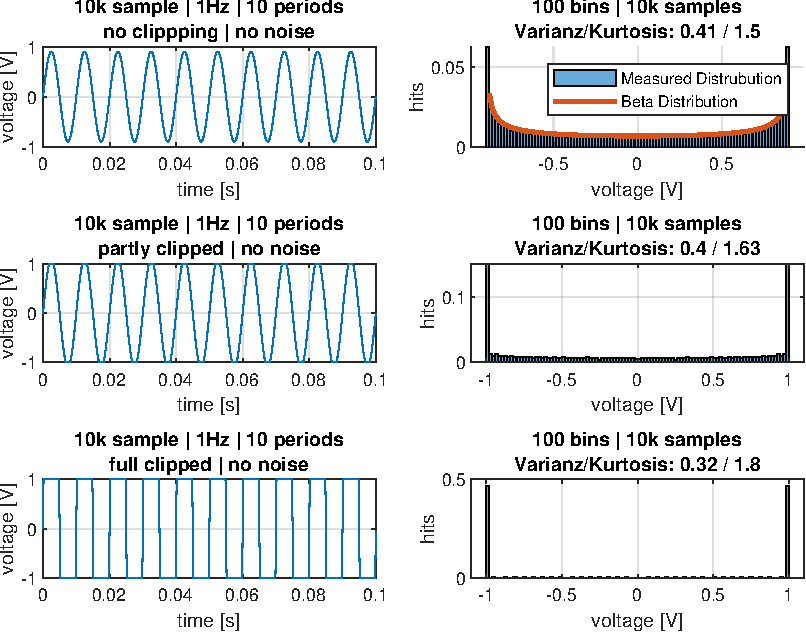
\includegraphics[width=0.7\columnwidth]{../../img/beta-distribution}}{\caption{Geometric parameters of a bolted joint.}\label{fig:rod}}	 
%				\end{figurehere} 
			\end{mdboxshad} 
\vspace{10mm}

			\begin{mdboxshad}
				{\textbf{Statistische Auswertung des Signals} erfolgt mithilfe der Auswertung der stochastischen Momente des Histogramms. Die stochastischen Momente werden verwendet, um Rückschluss auf die Signalqualität zu ziehen.
				Die Abbildung~\ref{fig:histo} zeigt die Verteilung der Datenpunkte im Quantisierungsraum des Analog-Digital-Wandlers (ADC). Bei verschiedenen Signalzuständen. Der Einfluss von Rauschen und Verstärkung ist  in der Verteilung deutlich zu erkennen.}
				\hspace*{2mm}
				\begin{center}
					\begin{figurehere}
						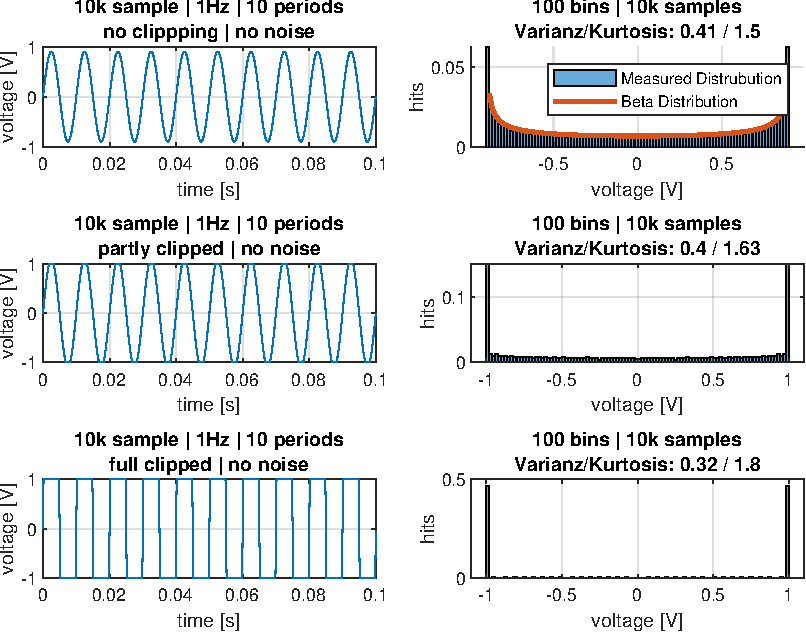
\includegraphics[width=0.45\columnwidth]{../../img/beta-distribution}~~~~~
						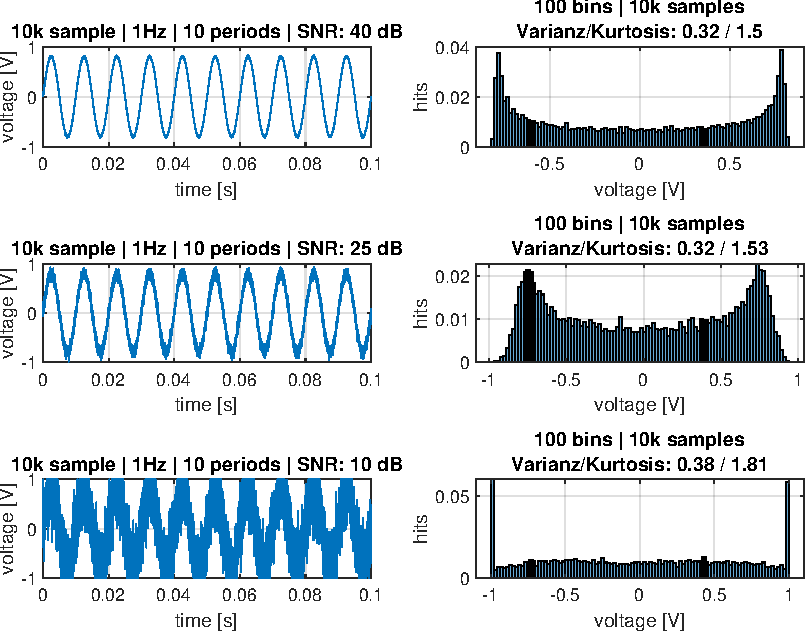
\includegraphics[width=0.45\columnwidth]{../../img/noise-histogramm}
						\caption{Die linken Histogramme werden durch rauschfreie Signale mit verschiedener Amplitude erzeugt. Dabei werden unterschiedliche Sättigungsgrade dargestellt. Die rechten Histogramme zeigen verschiedene Rauschverhältnisse bei konstanter Amplitude.}
						\label{fig:histo}	 
					\end{figurehere}
				\end{center}

			
				{\textbf{Ermittlung der Korrekturfaktoren} Der Zusammenhang der Korrekturfaktoren zeigt sich über den Störabstand und der Verstärkung des Signals mit den drei angeführten Größen: 
					\begin{itemize}
						\item Sättigungsgrad als Anteil der Datenpunkte in der Sättigung des ADC
						\item Varianz der Verteilung der Abtastwerte\footnote[1]{Nicht berücksichtigt werden Abtastwerte in der Sättigung des ADC.\label{foot:bereinigt}}
						\item Kurtosis der Verteilung der Abtastwerte\footref{foot:bereinigt}
					\end{itemize}
					Der Dynamikbereich des ADC ist in $b$ Stufen aufgelöst. Jeder Abtastpunkte kann in einem Histogramm einer Klasse $h_i$ zugeordnet werden, wobei $b \leq i$ ist. Der Sättigungsgrad ergibt sich aus der Anzahl der Abtastpunkte $n_0$ und $n_b$ in den äußersten Klassen $h_0$ und $h_b$ des Histogramms nach Gl.~\eqref{eq:dist_sat}.
					
					\begin{equation}
						\label{eq:dist_sat}
						c = \frac{n_0 + n_b}{n} \cdot 100
					\end{equation}
				}
				
			\end{mdboxshad} 
			\vspace{10mm}
			\begin{mdboxshad}
				
			\end{mdboxshad}  
			\columnbreak  
			\begin{mdboxshad}
			
			\end{mdboxshad} 
\vspace{10mm}
			\begin{mdboxshad}
			
			

			\vspace{-10mm}
			\end{mdboxshad} 
\vspace{10mm}
			\begin{mdboxshad}
				
			\end{mdboxshad} 
			\vfill
			\begin{mdboxshad}
				%\fontsize{26pt}{26pt}\selectfont
				\textbf{Förderung} Die Untersuchung entstand im Rahmen des Verbundprojekts 				ProMoBiS - "Progressive Multizell-Verbund-Konzepte für Batteriesysteme mit integrierter
				Sensorik". Das Forschungsprojekt wird vom Bundesministerium für Wirtschaft
				und Klimaschutz (BMWK) im Rahmen des 7. Energieforschungsprogramms (Förderkennzeichen
				03ETE046G) im Bereich " Energiewende im Verkehr" gefördert und vom Projektträger Jülich
				betreut.
			\end{mdboxshad} 
		\end{multicols}
		%\vfill
		%\par\noindent\rule{\textwidth}{0.4pt}
%		\vspace{-10mm}
		
		\vfill
%		\begin{multicols}{3}
%			\captionsetup{format=plain} 
%			\parindent0mm
%			\renewcommand*{\bibfont}{\fontsize{16pt}{16pt}\selectfont}
%			\selectlanguage{ngerman} 
%			\printbibliography
%		\end{multicols} 
		%\clearpage
	\end{document}
